\documentclass[../document]{subfiles}

\begin{document}
\section{Retired Architecture}
\label{retired_architecture}
\subsection{Introduction}
This chapter gives an overview of the system we had planned to implement, including quality attributes, architectural patterns, design patterns, tactics and architectural views. The purpose of this is to give an overview of the architectural structure of the system we first started to plan. We wanted to make a smart room where the we took in information from the sensors and used that information to create a better enviorment. We didn't start to make the logicview, developmentview and procesview until after we weren't going to create a smart room.

\subsection{Quality attributes}
\subsubsection{Functionality}
The system should function as planned. 

\subsubsection{Availability/reliability}
System should always be working, and be available 24h. Sensors might stop, but should have a time limit and restart when if it reaches the time limit. 

\subsubsection{Modifiability}
Our system needs to be easy to change/modify so our customer can expand and/or change the system afterwards. New sensors should be easy to implement.

\subsubsection{Usability}
User friendly, noobs should understand how to control the system, easy to modify custom settings.

\subsubsection{Portability}
Hardware should be easy to move to different environments and the system still works.

\subsubsection{Maintainability}
Customers should find it easy to maintain the system, the battery should be easy to change if battery is used, restart the system should be easy and maybe the system can restart itself if an error occurs. 

\subsubsection{Efficiency}
The system should be efficient and recognize relatively fast if the light is too bright, the temperature is too low/high to make a perfect environment in the room. 

\subsubsection{Security}
Depends on hardware. Other users who don't have authorization, should not be able to access our system.

\subsubsection{Scalability}
The system should be able to add more sensors/change scenery a.s.o.  

\subsection{Patterns and tactics}
\subsubsection{Model-View-Controller}
The Model-View-Controller (MVC) pattern is an architectural pattern that divides a software application into three interconnected components. The different components are the model, the view and the controller. The model manages the the application’s data, logic and rules. The view requests information from the model and uses this information to give an output representation of the information to the user. The controller takes input from the user and converts it to commands for the model or view. 

\subsection{Stakeholders and concerns}
\begin{table}[H]
	\caption{Stakeholders}
	\begin{tabularx}{\textwidth}{|X|X|}
		\hline
		\textbf{Stakeholders}	& \textbf{Descriptions} \\ \hline
		End user				& The end user is the future clients who will use our system.  \\ \hline
		Developers				& The developer are us in group 10 and our job is to develop the product and document the project.  \\ \hline
		Customer				& The customer is Stig Lau representing Altran AS. He will specify the product to be developed.  \\ \hline
		Advisor					& The advisor is Mohsen Anvaari. His job is to act as a project management.  \\ \hline
		Course staff			& The course staff for subject TDT4290 will provide information and prestudy for the course.  \\ \hline
		Hardware suppliers		& The hardware suppliers are the makers for the components used in this project.  \\ \hline
	\end{tabularx}
\end{table}

\subsection{Architectural views}
In this section we will show the different views of our architecture. We will follow the structure of the 4+1 View Model of Software Architecture. We chose this view model because this model allows us to handle the functional and nonfunctional requirements separately, and also address the different concerns of the various stakeholders separately.

\subsubsection{Logical view}				
The logical view is primarily concerned with the functional requirements. This means that it is concerned with what the system should provide in terms of services to its end-users. As we have changed the system 



\subsubsection{Development view}
The development view illustrates a system from a programmer's perspective and is concerned with software management. This view is also known as the implementation view. The software is packaged in small chunks that can be developed by one or a small number of developers. The subsystems are organized in a hierarchy of layers, each layer providing a narrow and well-defined interface to the layers above it. The development architecture of the system is represented by module and subsystem diagrams, showing the export and import relationships. 
 

\subsubsection{Process view}
The process view deals with the dynamic aspects of the system. It explains the system processes and how they communicate, and focuses on the runtime behavior of the system. The process view addresses concurrency, distribution, integrators, performance, and scalability, etc. UML Diagrams to represent process view include the Activity diagram.


\subsubsection{Physical view}
The physical view depicts the system from a system engineer's point of view. It is concerned with the topology of software components on the physical layer, as well as the physical connections between these components. This view is also known as the deployment view. The sensors are all somehow connected to the REST server, which gives information about the sensors to the database through the REST client. If the sensors for some reason are not used then the database gets random information from a data collector mock. Both the user interface and the command unit gets information from the database. The command unit is used to control the room. 

\begin{figure}[H]
	\centering
	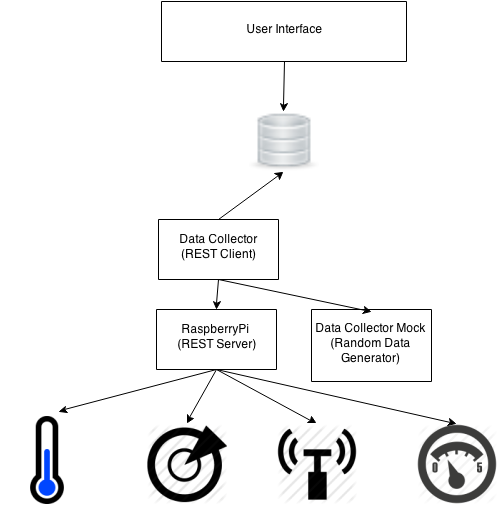
\includegraphics[width=\textwidth]{retierd_architecture/System_Diagram.png}
	\caption{System Diagram v.1}
\end{figure}

\subsubsection{Scenarios and use cases}
\paragraph{Scenarios} \ \\
The description of an architecture is illustrated using a small set of use cases, or scenarios which become a fifth view. The scenarios describe sequences of interactions between objects, and between processes. They are used to identify architectural elements and to illustrate and validate the architecture design. They also serve as a starting point for tests of an architecture prototype.

\begin{table}[H]
	\caption{Scenario P1}
	\begin{tabularx}{\textwidth}{|X|X|}
		\hline
		ID					& F1 \\ \hline
		Source				& System \\ \hline
		Stimulus			& Close the curtains when its too bright \\ \hline
		Environment			& Runtime \\ \hline
		Artifact			& Light sensors \\ \hline
		Response			& The curtains are closede \\ \hline
		Response Measure	& Time \newline Should be less than 5 minutes
		\\ \hline
	\end{tabularx}
\end{table}

\begin{table}[H]
	\caption{Scenario P2}
	\begin{tabularx}{\textwidth}{|X|X|}
		\hline
		ID					& F2 \\ \hline
		Source				& System \\ \hline
		Stimulus			& The user changes the temperature \\ \hline
		Environment			& Runtime \\ \hline
		Artifact			& Temperature sensors \\ \hline
		Response			& The temperature is changed \\ \hline
		Response Measure	& Time\newline Should be less than 5 minutes
		\\ \hline
	\end{tabularx}
\end{table}


\paragraph{Use cases} \ \\

\begin{figure}[H]
	\centering
	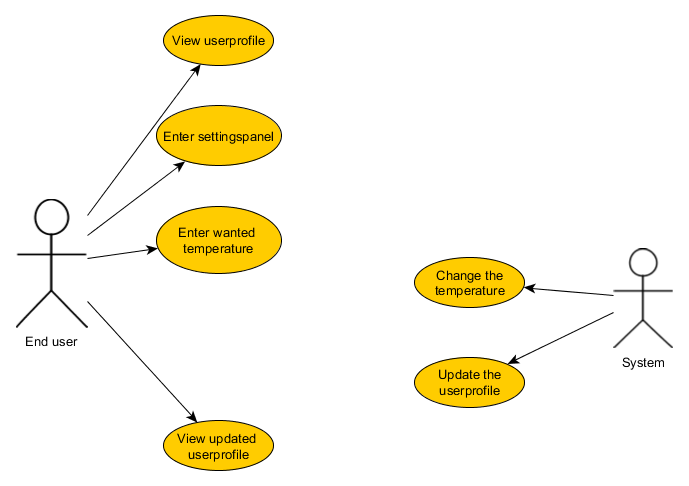
\includegraphics[width=\textwidth]{retierd_architecture/Usecase11.png}
	\caption{Use Case v.1.1}
\end{figure}

\begin{figure}[H]
	\centering
	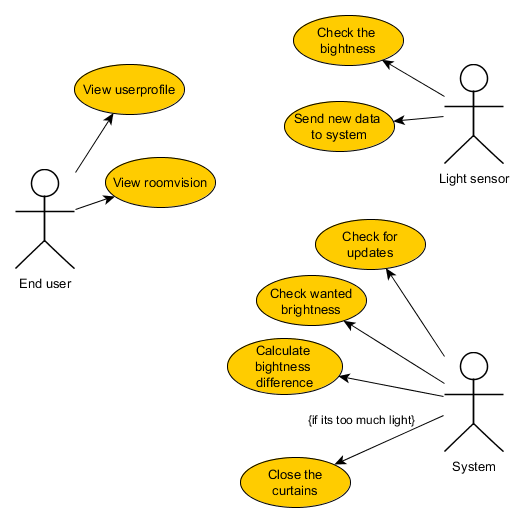
\includegraphics[width=\textwidth]{retierd_architecture/Usecase12.png}
	\caption{Use Case v.1.2}
\end{figure}

\subsection{Retierd Architectural views}
This section will cover the old views from when the visulizer was divided into three parts; the tableview, the historyview and the map view. 


\begin{figure}[H]
	\centering
	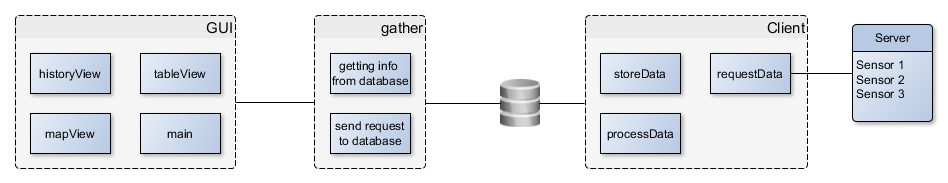
\includegraphics[width=\textwidth]{retierd_architecture/LogicalView1.png}
	\caption{Logical View v.1}
\end{figure}

\begin{figure}[H]
	\centering
	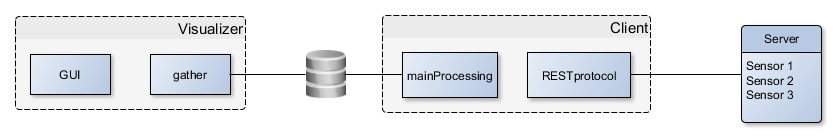
\includegraphics[width=\textwidth]{retierd_architecture/DevelopmentView.png}
	\caption{Development View v.1}
\end{figure}


\begin{figure}[H]
	\centering
	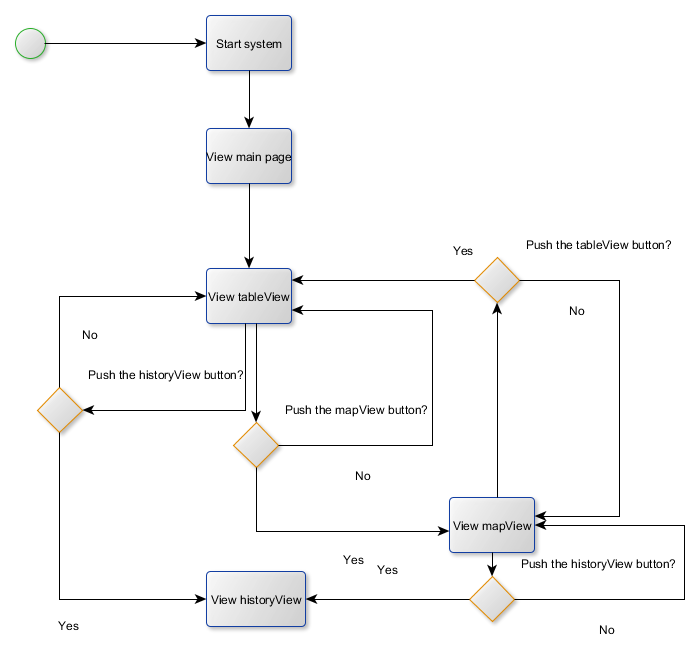
\includegraphics[width=\textwidth]{retierd_architecture/Processview1.png}
	\caption{Process View v.1}
\end{figure}

\begin{figure}[H]
	\centering
	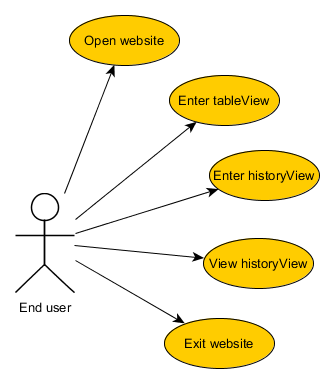
\includegraphics[width=\textwidth]{retierd_architecture/Usecase21.png}
	\caption{Use Case v.2.1}
\end{figure}




\end{document}